\chapter{Requirement Analysis}
\label{chap:requirement-analysis}

\section{Stakeholder Analysis}
\label{section:stakeholder-analysis}
% <TIP: List your stakeholders for your project here/>
% 
% Stakeholders are individuals, groups, or entities that
% have an interest, concern, or stake in a particular project, decision,
% organization, or system. These are individuals or groups who can affect or be
% affected by the outcomes of your project.

\subsection{Types of Stakeholders}
displays the categorization of stakeholders based on their power and interest in the project, using a matrix format to identify key groups and their level of influence and involvement.
\begin{table}[H]
    \centering
    \rowcolors{2}{white}{gray!5}
    \begin{tabularx}{\linewidth}{|l|X|}
        \rowcolor{gray!70}
        \hline
        \textbf{Type} & \textbf{Stakeholders} \\ 
        \hline
        \textbf{Internal Stakeholders} & Development Team, University Students, Professors, Academic Institutions \\ 
        \hline
        \textbf{External Stakeholders} & Investors, Educational Technology Companies, Potential Business Partners, Secondary School Students, General Public \\ 
        \hline
    \end{tabularx}
    \caption{Stakeholder Types}
    \label{tab:stakeholder-types}
\end{table}
\newpage
\subsection{Stakeholder Importance}
Table \ref{tab:stakeholder-importance} displays the categorization of stakeholders based on their power and interest in the project, using a matrix format to identify key groups and their level of influence and involvement.

\begin{table}[H]
    \centering
    \rowcolors{2}{white}{gray!10}
    \begin{tabularx}{\linewidth}{|l|X|}
        \rowcolor{gray!70}
        \hline
        \textbf{Importance Level} & \textbf{Stakeholders} \\ 
        \hline
        High Power, High Interest & Development Team \\ 
        \hline
        High Power, Low Interest & Investors, Educational Technology Companies, Potential Business Partners \\ 
        \hline
        Low Power, High Interest & University Students, Professors, Academic Institutions, Secondary School Students \\ 
        \hline
        Low Power, Low Interest & General Public \\ 
        \hline
    \end{tabularx}
    \caption{Stakeholder Importance Matrix}
    \label{tab:stakeholder-importance}
\end{table}

\newpage

\subsection{Stakeholder Analysis}
Table \ref{tab:stakeholder-analysis} provides a detailed stakeholder analysis, categorizing stakeholders based on their power, interest, and influence on the project.
\begin{table}[H]
    \centering
    \small
    \rowcolors{2}{white}{gray!10}
    \begin{tabularx}{\textwidth}{|>{\raggedright\arraybackslash}p{2.1cm}|>{\raggedright\arraybackslash}X|>{\raggedright\arraybackslash}X|>{\raggedright\arraybackslash}X|>{\raggedright\arraybackslash}X|>{\raggedright\arraybackslash}p{2.3cm}|}
        \rowcolor{gray!70}
        \hline
        \textbf{Name} & \textbf{Levels} & \textbf{Contact} & \textbf{Priorities} & \textbf{Impact} & \textbf{Strategy} \\ 
        \hline
        Development Team & High Power, High Interest & Internal Communication & System development and maintenance & Directly responsible for project success & Daily meetings, teamwork \\ 
        \hline
        University Students & Low Power, High Interest & University Network & Effective learning tool & Key users, provide feedback & User feedback sessions, surveys \\ 
        \hline
        Professors and Academic Institutions & High Power, High Interest & Academic Channels & Integration with learning & Influence on adoption & Collaboration, academic research \\ 
        \hline
        Investors & High Power, Low Interest & Business Meetings & Financial return & Provides funding support & Reports, presentations \\ 
        \hline
        Educational Technology Companies & High Power, Low Interest & Industry Contacts & Potential partnerships & Resource and tech support & Discussions, collaborations \\ 
        \hline
        Potential Business Partners & High Power, Low Interest & Business Network & Business opportunities & Scaling and market expansion & Networking, agreements \\ 
        \hline
        Secondary School Students & Low Power, High Interest & Educational Outreach & Future user base & Potential adopters & Awareness campaigns, trials \\ 
        \hline
        General Public & Low Power, Low Interest & Public Media & Awareness & Indirect impact & Social media, marketing \\ 
        \hline
    \end{tabularx}
    \caption{Stakeholder Analysis}
    \label{tab:stakeholder-analysis}
\end{table}

\section{User Stories}
\label{section:user-stories}

\subsection{Boss Battle Workflow}
\begin{itemize}
    \item As a high school student, I want to see my team’s progress in the boss battle, so that I can understand how much work is left.
    \item As a team leader, I want to assign tasks to my teammates, so that everyone has a clear responsibility.
    \item As a project manager, I want to view the team’s task flow, so that I can ensure an even workload.
    \item As a team member, I want to move tasks on the Kanban board, so that I can visually track my work.
\end{itemize}

\subsection{Success Meter}
\begin{itemize}
    \item As a university student, I want to see my individual performance score, so that I know how much I am contributing.
    \item As a team leader, I want to review my team’s overall performance, so that I can encourage struggling members.
    \item As a team member, I want to receive performance feedback based on my completed tasks, so that I can improve my work.
    \item As a team member, I want to earn badges for achievements, so that I feel motivated to complete more tasks.
    \item As a team member, I want to see a leaderboard ranking, so that I can compare my contributions with my teammates.
\end{itemize}

\subsection{Flow Track}
\begin{itemize}
    \item As a student, I want the system to estimate my risk of missing deadlines so that I can plan my time better.
\end{itemize}

\subsection{Target Users' Needs}
\begin{itemize}
    \item As a student, I want an easy system, so that I don’t waste time figuring it out.
    \item As a university student, I want a gamified task manager, so that group projects feel more engaging.
    \item As a high school student, I want a simple way to track group project tasks, so that I know what to do next.
\end{itemize}

% <TIP: Write user stories for each of your stakeholders here./>

% User stories are a technique used in agile software
% development to capture and describe functional requirements from an end
% user's perspective. They are a way of expressing software features or
% functionality in a simple, non-technical language that can be easily understood
% by both developers and stakeholders.

\section{Use Case Diagram}
\label{section:use-case-diagram}
<TIP: Write a use case diagram for your project here. Refer to an
article “What is a use case diagram?” by Lucidchart for help./>

\section{Use Case Model}
\label{section:use-case-model}
A use case is a detailed description of how a system
interacts with an external entity (such as a user or another system) to
accomplish a specific goal. Use cases provide a high-level view of the
functionality of a system and help in capturing and documenting its
requirements from the perspective of end users.

<TIP: Write use cases for your project here. Make sure to use the
appropriate type of use case for each scenario (brief, casual, and fully-dressed
use case)./>

\newpage
\section{User Interface Design}
\label{section:user-interface-design}
% <TIP: Put the initial design of your application here. You can
% showcase a detailed design of a specific page or a sitemap of your application.
% See an example below./>

\label{section:user-interface-design}

\begin{enumerate}

    \item \textbf{Home Page} \\
    As shown in Figure~\ref{fig:home}, this is the first page that the user lands on after logging in. It includes the user's profile, statistics, leaderboard, and their projects.    
    \begin{figure}[H]
        \centering
        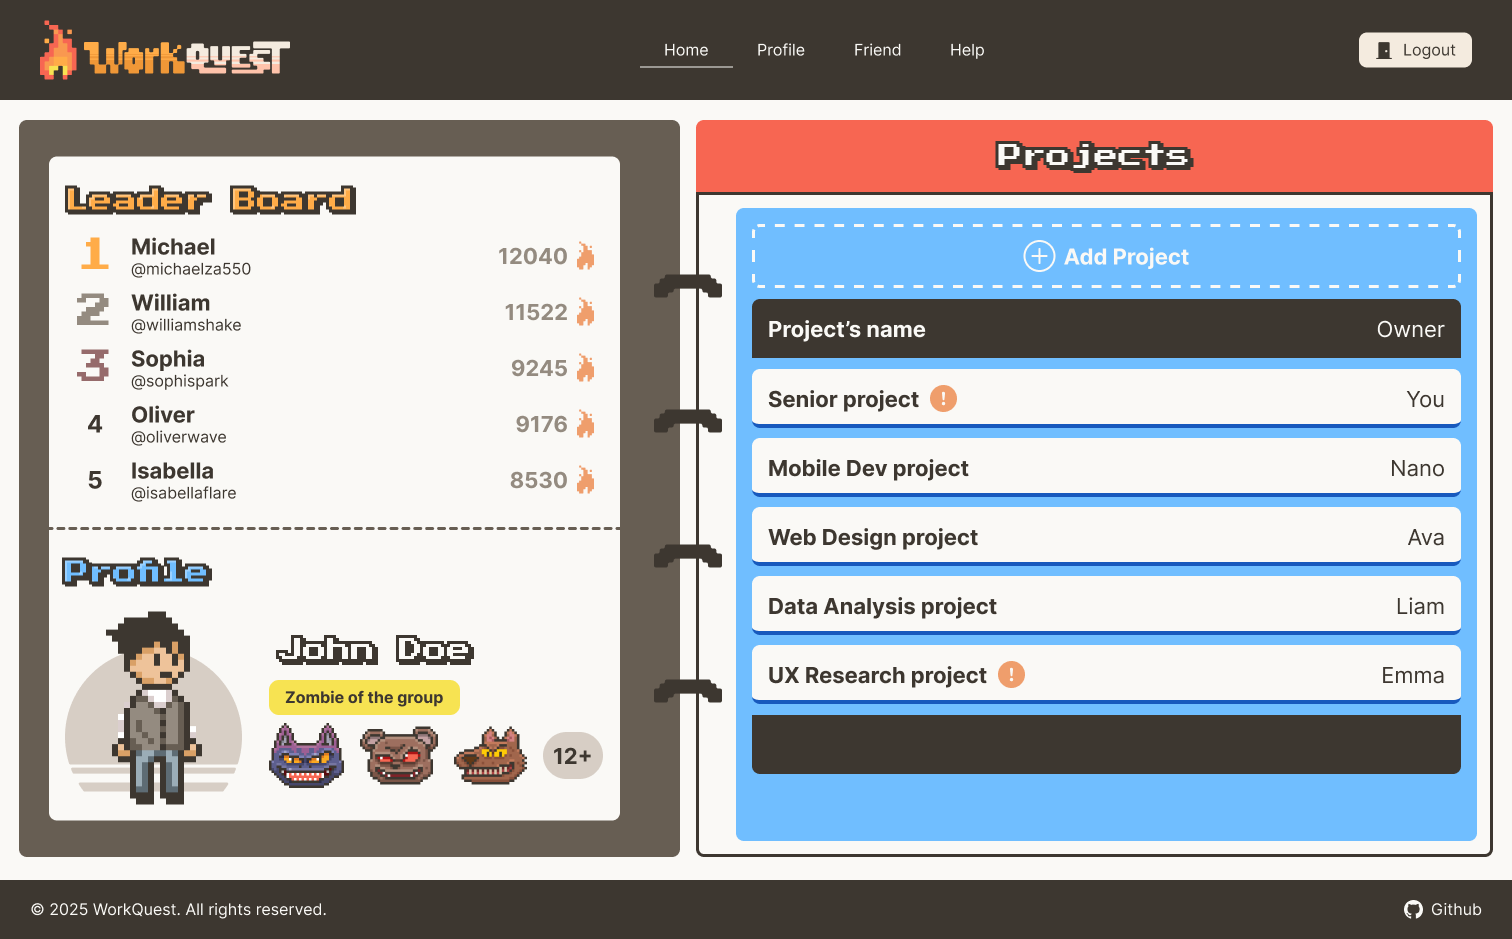
\includegraphics[width=0.5\textwidth]{mockups/Home.png}
        \caption{Home Page}
        \label{fig:home}
    \end{figure}
    
    \item \textbf{Project Page} \\
    As shown in Figure~\ref{fig:project}, this is the page where the user manages their projects while fighting a boss. It features a Kanban board and a boss graphic.    
    \begin{figure}[H]
        \centering
        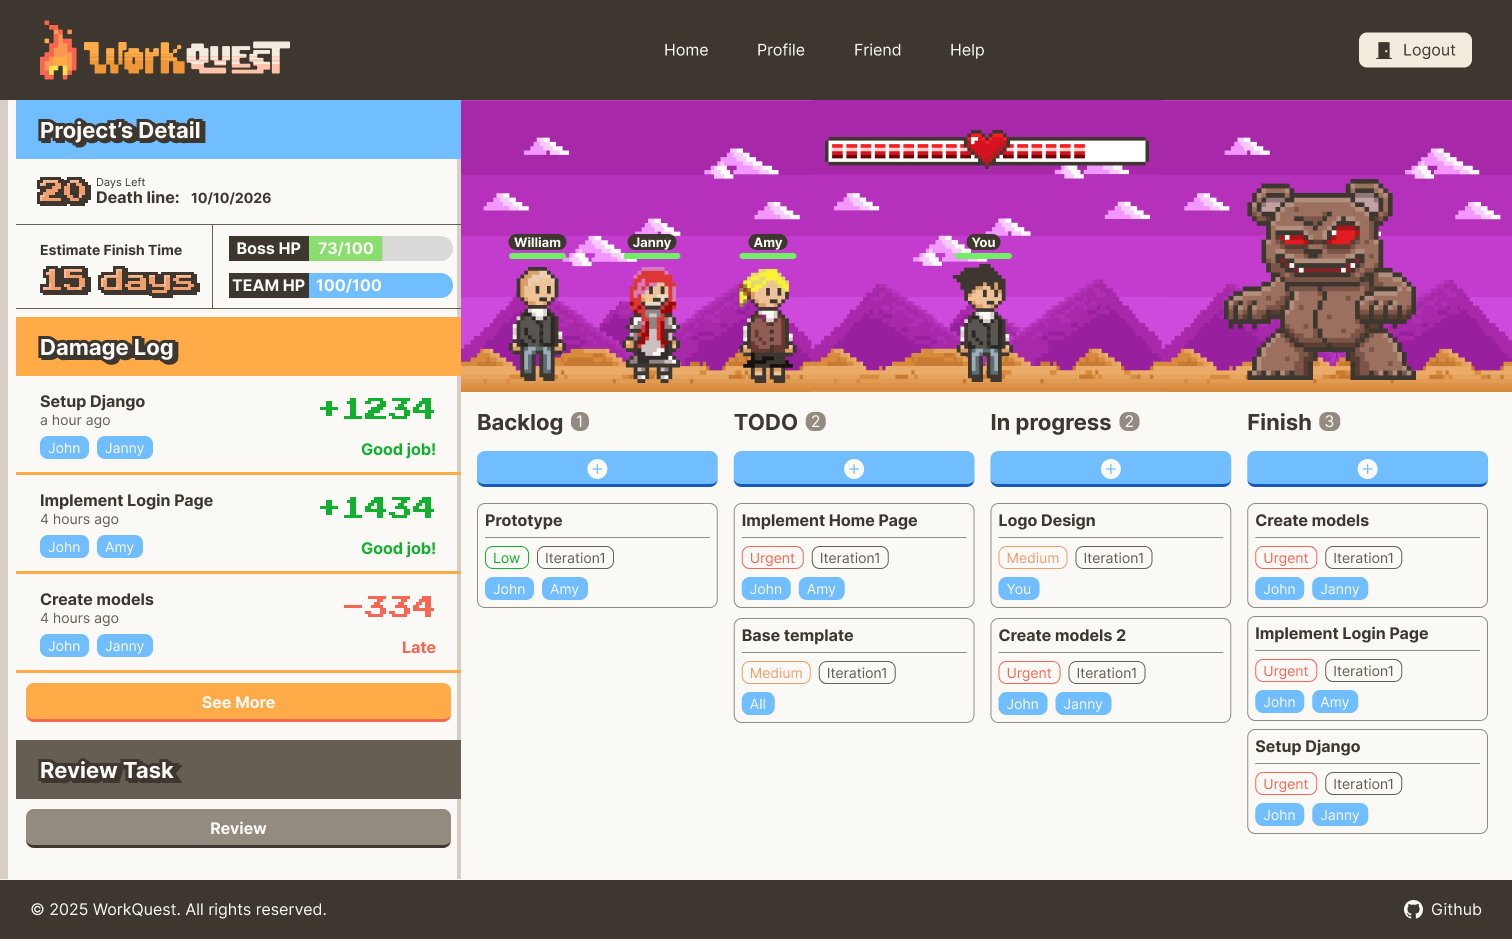
\includegraphics[width=0.6\textwidth]{mockups/Project.png}
        \caption{Project Page}
        \label{fig:project}
    \end{figure}
    \newpage

    \item \textbf{Feedback Page} \\
    As shown in Figure~\ref{fig:feedback}, this page is displayed at the end of the project. It visualizes all of the user's statistics, including boss fight performance, personalized feedback, and suggestions.    
    \begin{figure}[H]
        \centering
        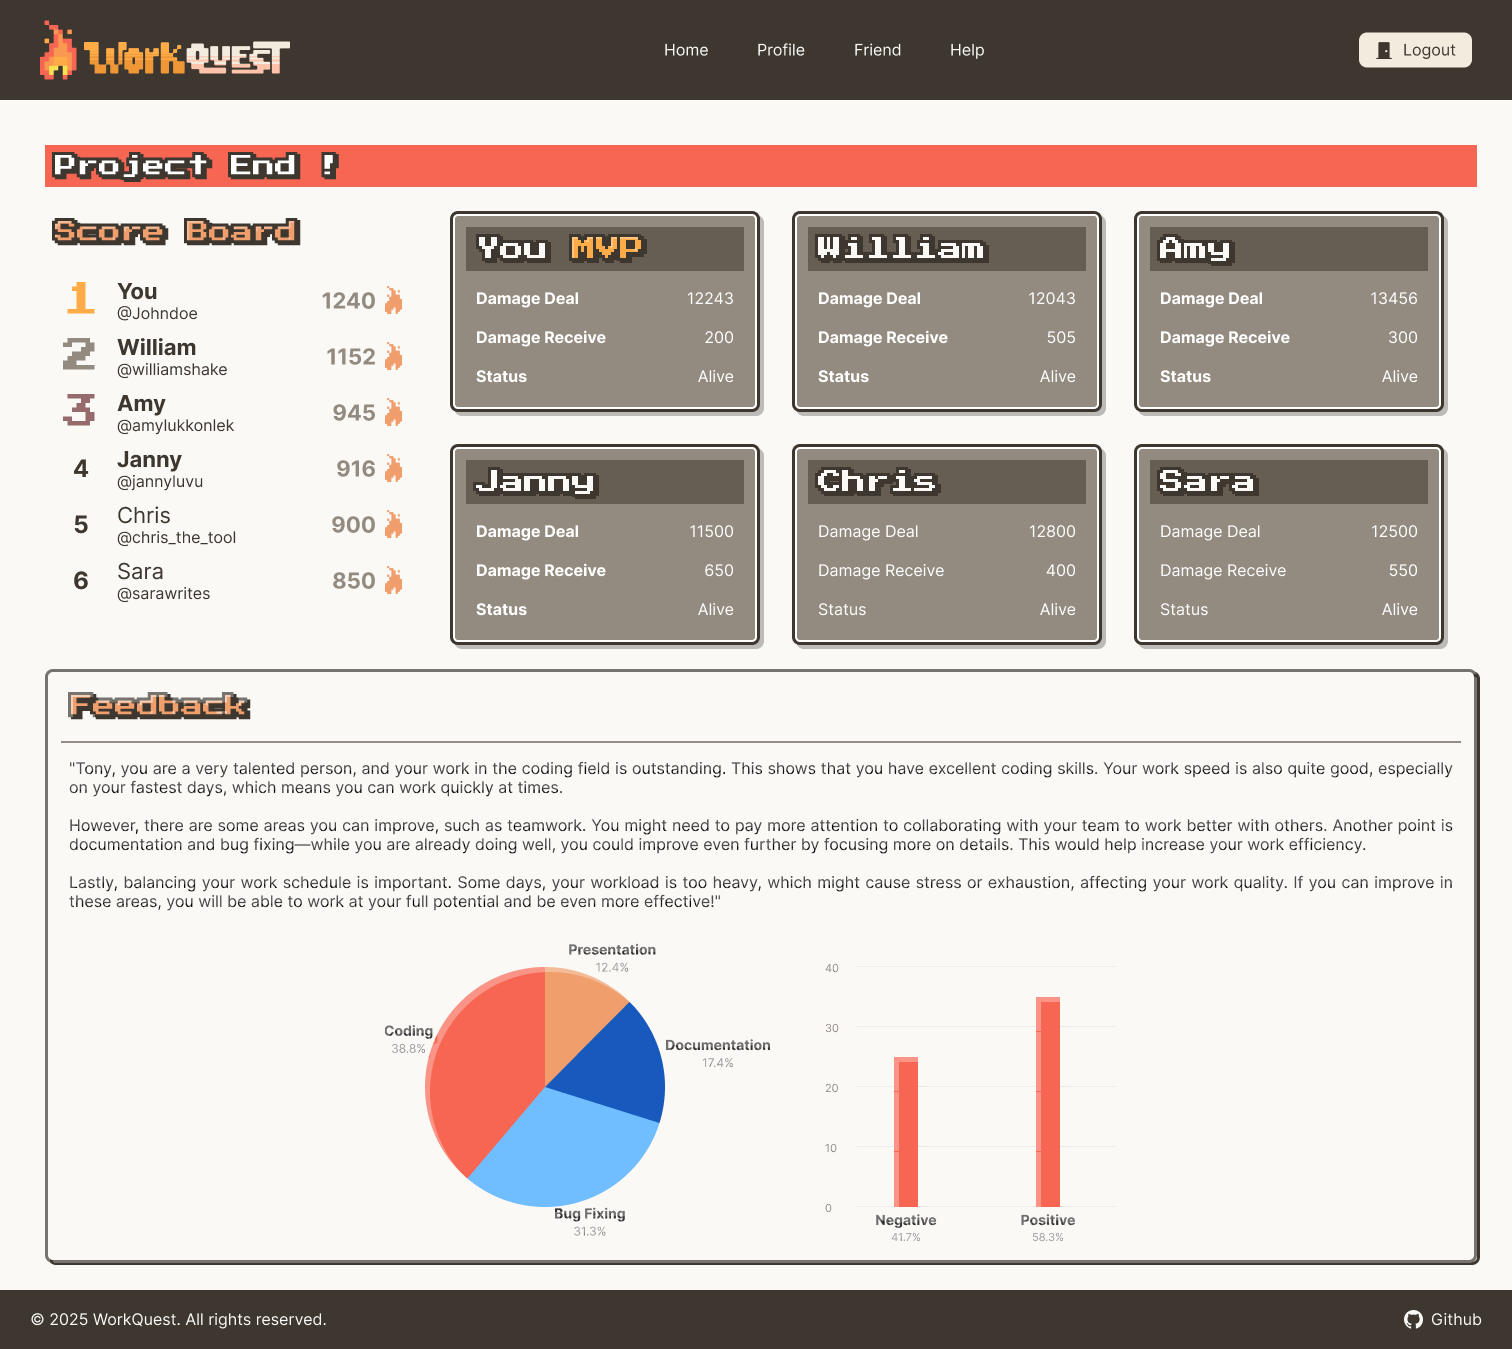
\includegraphics[width=0.5\textwidth]{mockups/Feedback.png}
        \caption{Feedback Page}
        \label{fig:feedback}
    \end{figure}

    \item \textbf{Dashboard Page} \\
    As shown in Figure~\ref{fig:dashboard}, this page shows your project statistics and progress, including a damage pie chart, estimated finish time, and a work speed time series.    
    \begin{figure}[H]
        \centering
        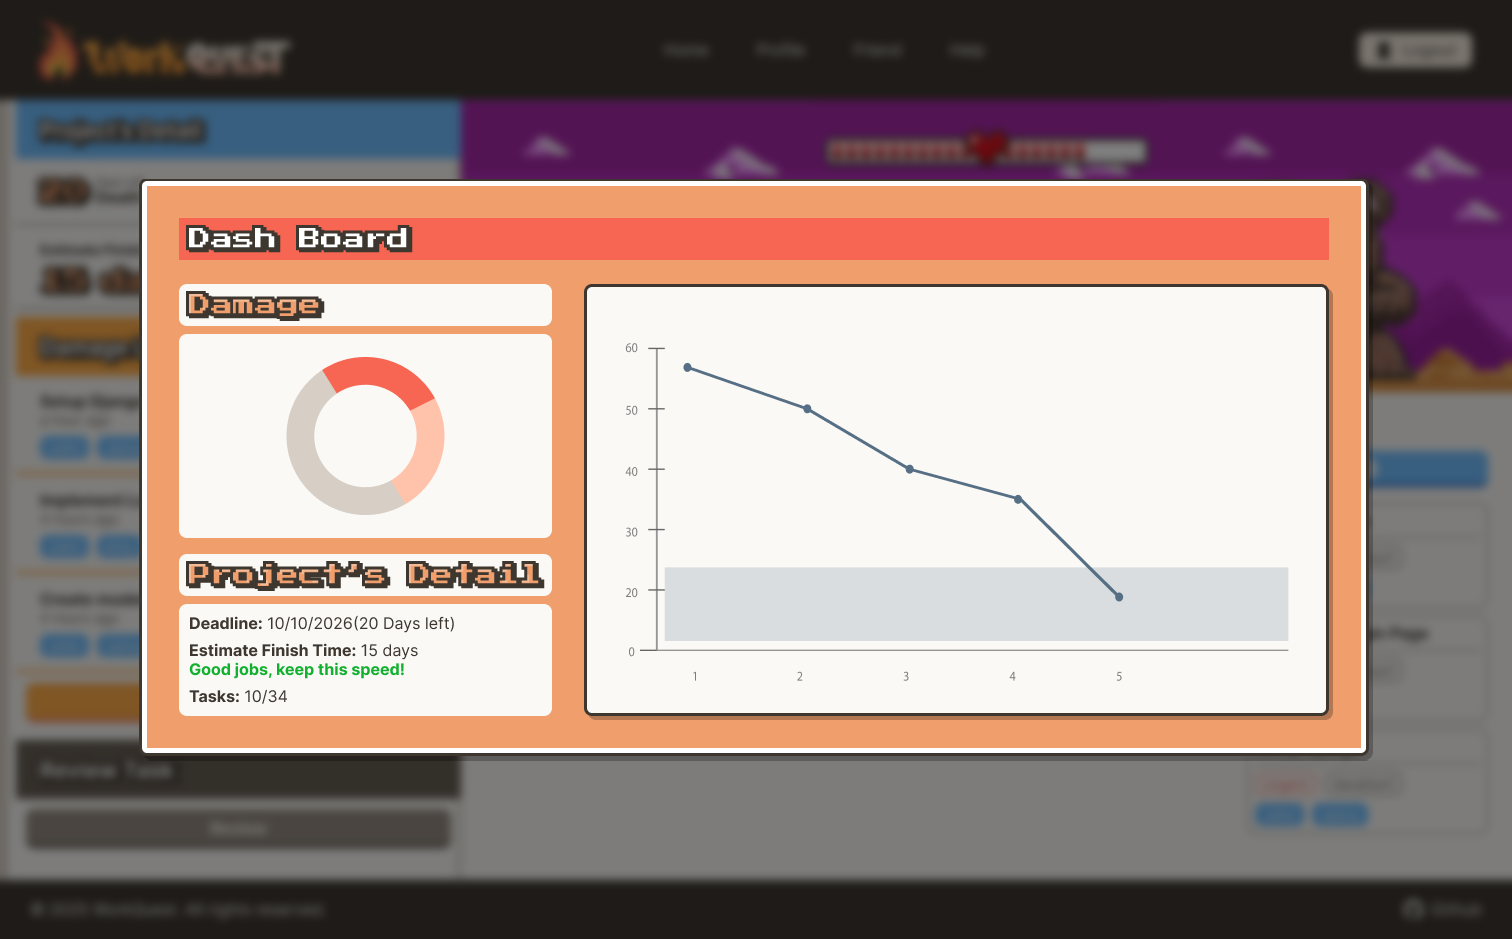
\includegraphics[width=0.6\textwidth]{mockups/Dash_Board.png}
        \caption{Dashboard Page}
        \label{fig:dashboard}
    \end{figure}

\end{enumerate}

% \begin{figure}[h]
%     \centering
%     \includegraphics[width=0.8\textwidth]{examples/user-interface-design.png}
%     \caption{User Interface Design}
% \end{figure}